
\section{Vergleich des impliziten und expliziten Euler-Verfahrens}

In diesem Kapitel geht es darum, die Auswirkung der impliziten Löser auf die \textit{NeuralODE} zu analysieren.
Dazu wurden drei Beispieltrajektorien berechnet.
Welche jeweils mit dem impliziten und expliziten Euler berechnet wurden,
um beide Verfahren möglichst gut miteinander vergleichen zu können wurde, darauf geachtet, dass beide Verfahren die gleichen Einstellungen haben.
Damit die expliziten Methoden
ihre Trajektorie komplett berechnen können, 
müssen die Fehlerwerte auf einen Mindestwert gesetzt werden.
Werden nun die Fehler der beiden berechneten Trajektorien
direkt miteinander verglichen, kann kaum ein Unterschied erkannt werden.
Deshalb wird in der Grafik \ref{fig:eulervergleich}
die Differenz der impliziten und expliziten Löser dargestellt.

$$
d = e_{Implizit} - e_{Explizit}
$$

Dabei wurde explizit auf den Betrag verzichtet, damit ersichtlich ist, in welchem Abschnitt welcher Löser den geringeren Fehler hat.
Ist die Differenz positiv, 
ist der explizite Euler besser.
Im negativen Bereich hat dann der impliziten Euler den geringeren Fehler.

\begin{figure}[H] 
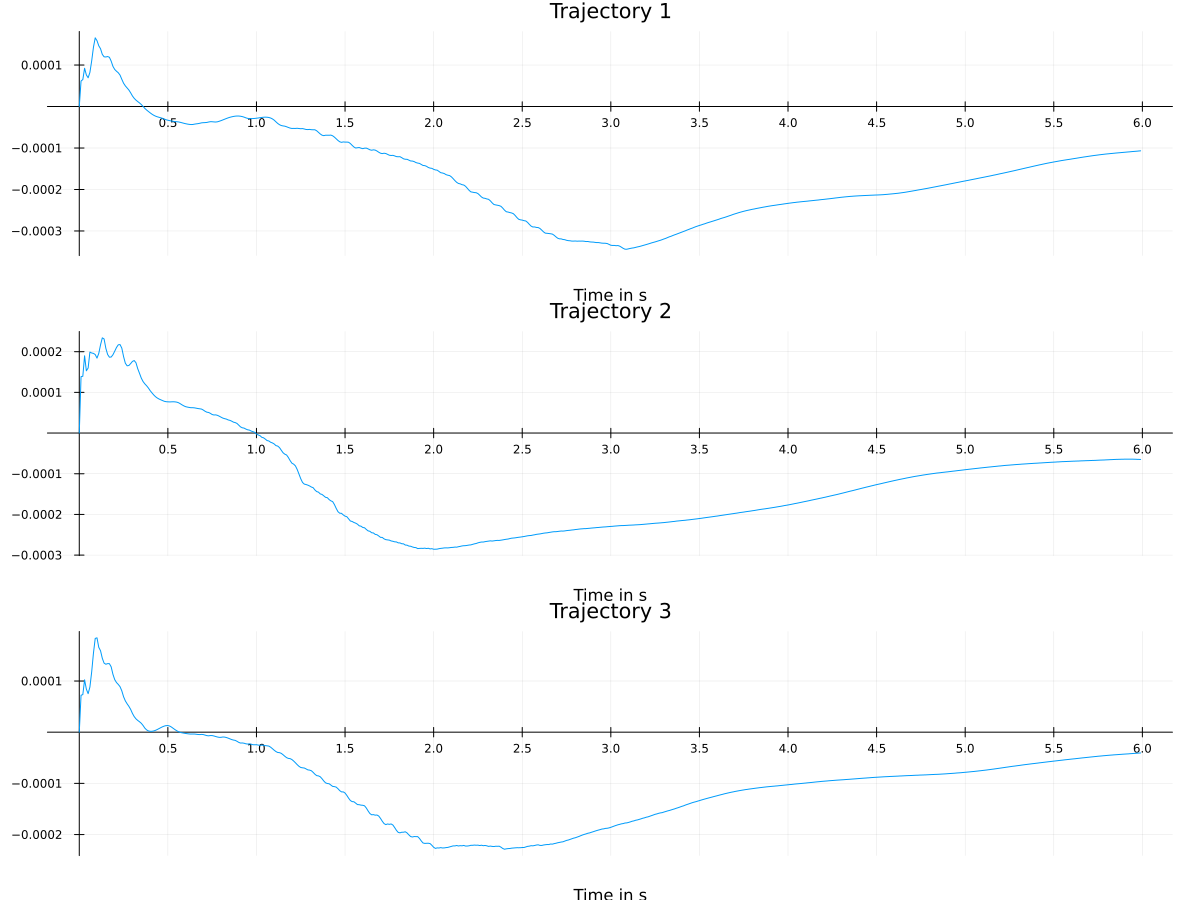
\includegraphics[width=0.9\textwidth]{Data/03_Ergebnisse/errors.png}
\caption{Vergleich von Impliziten und Expliziten Euler}
\label{fig:eulervergleich}
\end{figure}

In der Grafik \ref{fig:eulervergleich} kann beobachtet werden, dass bei allen Trajektorien zuerst der explizite Euler das bessere Ergebnis liefert.
Dies liegt vor allem daran, dass es sich in unserem Beispiel 
um eine Flüssigkeitssimulation handelt, welche mit einer laminaren Strömung beginnt.
Da diese sich sehr linear verhalten, liefert der expliziten 
Euler hier äußerst gute Ergebnisse.
In der Simulation trifft das Wasser dann nach 0,5 s bis 1 s
auf ein Objekt.
Dies sorgt für mehr Turbulenzen im Fluss der Flüssigkeit.
Ab diesem Zeitpunkt ist der implizite Euler besser.
Dies liegt vor allem daran, dass dieser mit nicht linearen Problemen besser zurechtkommt.
Es fällt außerdem auf, dass sich beide Verfahren mit der Zeit
immer weiter annähern.
Dies liegt daran, dass im Allgemeinen mit der Zeit die Fehler der
Trajektorien immer größer werden.
Auch wenn es anhand der Daten nicht zu erkennen ist,
lassen die Daten vermuten, dass der implizite Euler auch bei längeren Trajektorien ein besseres Ergebnis liefert.
Der große Unterschied zwischen den zwei Verfahren ist die Laufzeit.
Bei den expliziten Methoden kann eine Laufzeit von ein paar Minuten 
erwartet werden. Beim impliziten Euler kommt es zu einer Laufzeit von einigen Tagen. 
Im nächsten Kapitel wird gezeigt wie, die beiden Verfahren miteinander 
verbunden werden können.

